\chapter{No innovation without data}\label{ch:mlbasics}

The area of \gls{ml} have evolved significantly over the past decade. This development and progression are partly due to the increased availability of computing resources and open-source libraries. Applying\gls{ml} in the year of 2020 is no longer limited to knowledgeable mathematicians/software engineers that are well-versed within the field. Drag-and-drop type interfaces for the non-programmer are even available through services such as Amazon Web Services making it access-able to everyone interested. \gls{ml} have been shown in recent years to improve specific tasks, and solve complex problems. For instance, massive performance gains have been achieved in computer vision and speech recognition tasks. For example, Google Translate is no longer many million lines of code. It is reduced to an adaptive model that has learned from many experiences \cite{Wu2016GooglesTranslation}. So not only has \gls{ml} reduced the complexity of solving the problem, but it has also improved the performance of such a system quite significantly. The most significant gains can, however, be seen in the area of computer vision. State-of-the-art \gls{ml} algorithms can surpass human performance in tasks such as image classification. Stories such as these, and many others, have caused \gls{ml} to find its way to mainstream media. \gls{ml} also termed \emph{\gls{ai}} is foreseen to be the solution to many complex problems where we as humans have great difficulties engineering solutions. However, such solutions come at the cost of transparency. Many \gls{ml} models provide solutions that even the engineers constructing them do not understand. This lack of transparency has increased with the recent introduction of \gls{dl}, a sub-field of \gls{ml} that learns from raw data. These models can have many millions of parameters, and the solution they offer can be challenging to interpret. 

The purpose of this chapter is to outline standard terms associated with the field of \gls{ml} as used throughout this dissertation.



\section{Machine Learning basics}

The tools of \gls{ml} is separated into different families of learning. These are known as \emph{supervised}-, \emph{unsupervised}-, and \emph{reinforcement} learning. Each of these families has different approaches to modelling and is summarised below. 

\paragraph{Supervised Learning}

Is considered the primary and most successful area of \gls{ml}. Supervised learning attempts to construct a mapping function between input $x$ and output $y$ through a function $f(\cdot)$. Thus the task of supervised learning is to find a function $f(\cdot)$ that can map between $x$ and $y$. To formulate a supervised learning problem, input data, as well as observations, are required. 

\paragraph{Unsupervised Learning}

Attempts to learn the underlying function of the data. Thus the task is to find a lower-dimensional latent variable such that the input can be represented by a function $f(\cdot)$ and a latent variable $z$. Subsequently, unsupervised learning is applied where no observations are available, but the data in itself contains information that may be challenging to represent \cite{M.Bishop2006}.

\paragraph{Reinforcement Learning}

Is the idea of learning through feedback. Reinforcement Learning systems are tasked with learning optimal policies. Policies can be defined as taking the \emph{correct} action given a specific state/observation of the system to optimize. Through interacting with the system/environment, the policies are optimized with respect to a reward metric. The metric is to reward or penalize the reinforcement learning system if a good or bad action is taken for a given observation. Over trial and error (i.e. iterations) such a reinforcement learning system learns the optimal policies and will provide the actions that maximize the reward. 

\subsection{Iterative learning}
The learning process in \gls{ml} methods differs significantly from tool to tool. The primary tools used throughout this dissertation are based on iterative algorithms, as commonly associated with such \gls{ml} models as \gls{nn}. It should be noted that not all \gls{ml} tools are based on iterative learning processes. \emph{Classic} \gls{ml} tools are based on analytical mathematics that uses all available observations for computing and learning. Such models as \gls{nn} use an iterative approach to learning from the data. This approach offers not only performance improvements for large datasets but also feasibility in terms of computational runtime. Iterative learning can be shown to be capable of converging towards optimal solutions in both convex and non-convex problems \cite{M.Bishop2006}. A simple example of adaptive iterative learning is attempted given below:

\emph{Adaptive filters} is a relatively intuitive example of iterative learning and can be found in most modern electronic devices. As to whether adaptive filters can be defined as \gls{ml} is up to the reader. However, many of the same principles associated with \gls{ml} are employed. 

The purpose of adaptive filters is to find a filter that approximates a dynamic and unknown system. In mobile communication, such an adaptive filter is available at the receiver in an attempt to \emph{equalize} the changes imposed by the wireless channel. Such a tool is also known generally as an \emph{equalizer} and can be found in most communication systems. The problem in wireless communication is the dynamic and unknown channel; we call it $H$. The channel imposes distortions and noise to the transmitted and originated waveform. With the presence of noise and distortions caused by the channel, the original signal must be extracted to enable and construct a communication system. For this, an adaptive filter is commonly used.  As shown in Fig. \ref{fig:adaptive_filter_system}, the purpose of the adaptive filter is to approximate the channel response $H$. An adaptive filter can be formalized as a \gls{fir} filter and takes the form 

\begin{equation}\label{eq:fir}
    y[n] = \sum_{i=0}^N w_n[i]x[n-i]
\end{equation}

Where $y[n]$ is the samples at the output of the system in time, $w_n$ are the filter weights with a finite number of weights, and $x_n$ are the samples at the input of the system. Thus, the objective is to find the coefficients/weights of $w_n$. 

\begin{marginfigure}
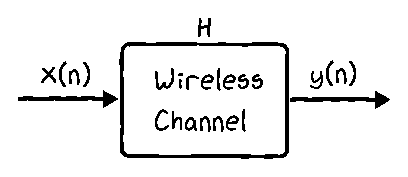
\includegraphics[]{chapters/part_pathloss/figures/adaptive_filter.eps}
\caption{The wireless channel can be seen as a dynamic system. The task at the receiver is to \emph{equalize} the channel conditions, e.g. approximate the response $H$ such that more of the originated signal $x(n)$ can be recovered by $Y = X*H$ thus $X = Y/H$.}\label{fig:adaptive_filter_system}
\end{marginfigure}

A so-called \emph{Weiner filter} is capable of solving such a system. Nevertheless, it requires the so-called inverse auto-correlation, which is computational heavy \cite{Tan2013DigitalProcessing}. More so, the auto-correlation function is based on statistics; therefore, a significant number of samples are required. To combat the complexity of such a filter, an adaptive filter using a \gls{lms} with steepest descent can accurately approximate an optimal filter using iterations. The weights of the filter are updated such that they converge towards the optimum weights. Such a steepest descent can essentially be termed a gradient descent algorithm, which uses the gradient of the error to update the weights. The weight update equation can be seen as
\begin{equation}
    w_{n+1} = w_n - \mu \nabla  \epsilon [n]
\end{equation}

Where $\mu$ is a converging factor, and $\nabla  \epsilon [n]$ is the gradient of the mean-squared error between the output of Eq. (\ref{eq:fir}) and the true observations of the channel. The update equation adjusts the weight by considering the error, and the direction of it. $\mu$ is the step-size of updating the coefficients and is an important parameter for controlling convergence complexity. Updating the weights in this way is essentially the same principle used for updating weights in \gls{nn}. An example of an equalizer applied to a signal in mobile communication can be seen in Fig. \ref{fig:equalizer_example}. The filter successfully corrects phase and amplitude to effectively \emph{cancel out} the imposed channel impairments.

\begin{figure}
    \centering
    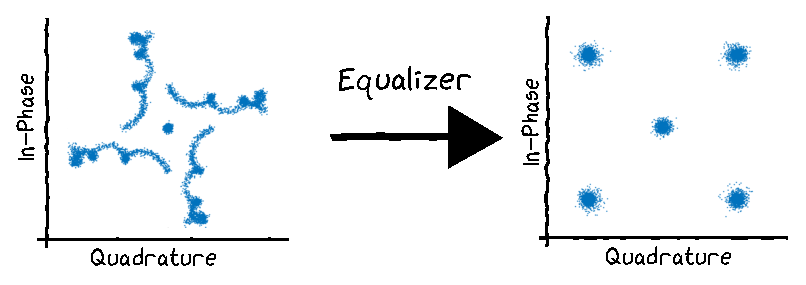
\includegraphics[width=\textwidth]{chapters/part_pathloss/figures/equalizer_example.eps}
    \caption{A received signal under impairments can be seen on the left-hand side. The equalizer is tasked with identifying the channel coefficients through the weight update procedure. The resulting constellation diagram of \gls{qpsk} symbols can be seen on the right-hand side. }
    \label{fig:equalizer_example}
\end{figure}

\subsection{Neural Networks}\label{sec:neural_networks}

Neural Networks are essentially a collection of adaptive weights that are connected, similar to how an \emph{adaptive filter} is constructed. However, one key difference is the use of non-linear transformation functions on said weights (also known as activation functions). \glspl{nn} are highly flexible and is capable of approximating any continuous function in $\mathbb{R}^n$ \cite{Nielsen2015}. This property makes them incredibly useful for many complex problems. The purpose of this section is to provide the reader with basic principles related to \gls{nn}. More details, proofs, and applications can is found in references such as \cite{Nielsen2015}, \cite{M.Bishop2006}.

A two-layer \gls{nn} can be written in the form.

\begin{equation}\label{eq:neural_network}
  y_k(\mathbf{x},\mathbf{w}) = \sum_{j=1}^M w_{kj}^{(2)} h\left( \sum_{i=1}^D w_{ji}^{(1)}x_i+w_{j0}^{(1)} \right) +w_{k0}^{(1)}
\end{equation}

Where $y_k$ is the kth output given a number of inputs $\mathbf{x}$ and a set of weights $\mathbf{w}$, each layer consists of a finite number of weights, in case denoted by $D$ and $M$ for layer (1) and (2) respectively. $h(\cdot)$ can be seen as any transformation function, also termed an \emph{activation} function. The weights are updated using a \emph{loss} function that seeks to compute the error between the predicted $y_k$, and the observed $y_k$. For example, for a single output $y$, with $n$ observations we can write a sum of squares as follows.


\begin{equation}\label{eq:sum-of-squares}
  E(\mathbf{w}) = \frac{1}{2}\sum_{n=1}^N ||y_n(x_n,\mathbf{w}) - t_n ||^2
\end{equation}

In this particular case, the observation is denoted $t_n$. Such a loss function is commonly used when dealing with continuous observations. Different loss function exists for various purposes. However, the principle of minimizing the loss with respect to the weights $\mathbf{w}$ is similar regardless of the loss function used \cite{M.Bishop2006}. For the sum-of-squares error function, as shown in Eq. \ref{eq:sum-of-squares}, it can be shown that maximizing the likelihood function is identical to minimizing the sum of squares. The task is to find a point in the weight space $w$ where the gradient of the error function is zero thus $\nabla E(w) = 0$. However, due to the non-linearities imposed by the function $y_k(\cdot)$ finding an analytical solution is not feasible. For these reasons, the update of weights in \gls{nn} use an iterative approach, much like the adaptive filter. For cohesion, the weight update equation for \gls{nn} in its simplest terms can be written as

\begin{equation}\label{eq:weight_update}
    w_{\tau + 1} = w_{\tau} - \eta \nabla E(w_{\tau})
\end{equation}

In \gls{nn} terms, we can see this as utilizing the gradient information by stepping in the direction of a negative gradient. $\eta$ is known as the \emph{learning rate} and determines the step size. Several techniques for utilizing gradient information exist. The primary difference is related to how large batches of data is iterated over. The two primary principles used throughout this dissertation is:

\paragraph{Stochastic gradient descent}
is also known as an online gradient descent method that seeks to update the weights based on one data point at a time.

\paragraph{Mini-batch gradient descent}
Unlike traditional batch methods such as \emph{steepest descent}, the utilization of mini-batches splits the training set into smaller batches hence \emph{mini-batch}. Mini-batch training has shown to stabilize training and improve convergence time. \cite{Nielsen2015}.

The gradient information is relatively easy to utilize, if and only if, one can compute the gradient with respect to the weights for all weights in \gls{nn}. Even for a two-layered \gls{nn}, a problem arises. It is only possible to measure the error at the output layer; thus, the first layer requires information from the last layer. Here is where the idea of \emph{back propagation} comes into play. Backpropagation is a technique for passing messages backwards through \gls{nn}. It can be shown that by applying the chain rule, we can construct a method for moving around the necessary gradient information. Such a proof can be found in references as \cite{Nielsen2015, M.Bishop2006}. In short, the backpropagation procedure consists of 1) Applying an input to the network and forward propagate the entire network. 2) For all outputs, the derivative of the error is evaluated. 3) the \emph{errors} is propagated backwards such that a derivative is obtained for all hidden units. 
 



\subsection{Training, test and validation}
Learning any model requires separate datasets for training and testing the model to avoid such factors as over and underfitting. If the complexity of the model is higher than what is required for learning the underlying function, it results in learning of the noise present in the dataset instead of the characteristics of the problem, which is usually not desired and is also termed overfitting. If the model is simpler than the function to be learned, the model will not provide effective predictions and is termed underfitting. A comprehensive and detailed introduction to such overfitting and underfitting terms and how it relates to model complexity can be found in \cite{M.Bishop2006}. To test and validate the performance of a trained model the data is split into separate datasets. Some of the data is thus kept unseen to the model when trained. Over time and experiments, it is unavoidable to develop some kind of bias for a particular dataset, regardless of it being seen or not during training. Thus, the more data available, the more validation is possible. A few common tricks of the trade can be used to increase data quantities, such as \emph{data augmentation} (See \ref{sec:regularization}) or \emph{cross-validation}, the objective being the same; improve performance of the model for unseen combinations of features and targets. In other words, separate datasets are required for validating if the underlying characteristics of the problem have been learned and if the model is well-tuned.

\subsection{Optimizers}\label{subsec:optimizers}
Several techniques for gradient descent have been developed over recent years to deal with training issues and improving training speed. A vital concern of traditional stochastic gradient descent is getting stuck in local minima in the cost function space, which restricts the training performance significantly \cite{Goodfellow-et-al-2016}. Optimizers that improve training performance and avoid or can get unstuck from local minima have been used throughout this dissertation, such as Adam, and L-BFGS \cite{Goodfellow-et-al-2016}. 

\subsection{Regularization}\label{sec:regularization}
The common way of reducing over-fitting of trained models is by introducing regularisation. A simple way is by adding a regularisation term to the cost function as given in Eq. (\ref{eq:sum-of-squares}) such that

\begin{equation}
    E(\mathbf{w}) = \frac{1}{2}\sum_{n=1}^N ||y_n(x_n,\mathbf{w}) - t_n ||^2 + \underbrace{\frac{\lambda}{2} \mathbf{w}^T \mathbf{w}}_{\texttt{weight decay}}
\end{equation}

This scales the loss by the weight vector and a parameter $\lambda$ and essentially encourages the weight values to decay towards zero, which has been termed \emph{weight decay} in literature. Several functions for regularisation can be added to the cost function, and such approaches are commonly termed \emph{L1} and \emph{L2} regularisation, depending on the specific term used for the weight decay. However, the purpose is identical, to force or encourage the weights towards zero. However, if too much weight decay is added the issues of under-fitting might arise. It is thus an essential hyper-parameter in the training of any \glspl{nn}.

\paragraph{Dropout}
Regularisation can also be introduced by several techniques directly embedded into the structure of the model. Examples of such layers are, drop-out and batch normalization (See section \ref{subsec:dropout} and \ref{subsec:batch_normalization})

\paragraph{Data Augmentation}
Introducing noise into the data set can also be seen as a regularisation technique as it generates an increase in the quantity of available data. The random noise ensures the model does not memorize the data points as the overall noise present on the observations is increased, which effectively reduces over-fitting and ensures the model converges towards the underlying function capable of characterizing fundamental properties of the data. Such techniques have successfully been applied to image modelling tasks by introducing random rotations on the original input images \cite{Shorten2019ALearning}. Engineering effective data augmentation techniques are considered a challenge for many supervised modelling problems. 

\subsection{Definitions}
The world of \gls{ml} consists of a particular set of terminology. This section will attempt to summarise some of the primary language and notations used throughout the dissertation.

\paragraph{Features}
The term \emph{input} is used interchangeably with \emph{features} to define the variables given to the model. In the world of statistics, such might also be termed predictors or regressors. As a rule of thumb, we define \emph{features} as engineered inputs and is commonly the primary input variable given to classical \gls{ml} methodologies. In \gls{dl}, raw data is processed through deep layered structures to produce \emph{features}. In this case the input variables to \gls{dl} models are by default termed \emph{inputs}. 

\paragraph{Targets}
The terms \emph{target} and \emph{output} are used interchangeably throughout this dissertation. In the world of statistics, this is also known as \emph{response} variables. 

\paragraph{Layers and Depth}
\gls{nn} utilize layers (or hidden layers) to process features and inputs. Layers consist of adaptive weights termed \emph{neurons}. Each layer in \glspl{nn} has thus a certain amount of neurons. A sequence of layers determines the depth and size of the \gls{nn}. In practice, any \gls{nn} with more than two layers is considered a \gls{dnn}, however, used for different purposes and with different inputs \cite{M.Bishop2006}. Thus when refereed to the \emph{depth} of the model, it is the number of sequentially connected layers. 

\paragraph{Generalization}
The term generalization describes how well a trained model is capable of generalizing the underlying characteristics and functions of the problem. In practice, generalization is seen as the gap between training and test losses - also known as the \emph{generalization gap}. 

\subsection{Implementation}
The research of applying and studying \gls{ml} and \gls{dl} methods are contingent on the ease of implementation. Several toolboxes are made available, (either open-source or under license) that ease the efforts required for implementation. For instance, MathWorks, has spent efforts towards designing drag-and-drop \gls{gui} for constructing \gls{dl} models with \gls{gpu} acceleration. that enables the creation of complex models by everyone interested. A few of these toolboxes have been utilized throughout the research documented in this dissertation. Initial models were implemented with Tensorflow \cite{tensorflow2015-whitepaper}. For later and improved implementations, Pytorch \cite{Paszke2017AutomaticPyTorch} was utilized. The Deep Reinforcement Learning was completed using the \cite{MATLABRL_toolbox}. The different implementations do in practice mean different results. However, due to the large communities maintaining these toolboxes, it is believed that performance, regardless of the toolbox used, is comparable. 

\subsection{Evaluation Metrics}\label{subsec:eval_metrics}
The metric of evaluating the training and test loss depends on the model architecture. However, a set of well-known metrics can be used for assessing the performance of the proposed approach. Here $\hat{y_i}$ are the predicted values of the model, while $y_i$ are the true values.

\begin{equation}
    MSE =  \frac{1}{N} \sum_i^N (\hat{y_i} - y_i)^2
\end{equation}

\begin{equation}\label{eq:rmse}
    RMSE = \sqrt{\frac{1}{N} \sum_i^N (\hat{y_i} - y_i)^2}
\end{equation}

\begin{equation}
    MAE =  \frac{1}{N} \sum_i^N |\hat{y_i} - y_i|
\end{equation}


\section{\acrlong{dl} Basics}\label{sec:dlbasics}

\gls{dl} is essentially considered an extension of \gls{ml} and utilize a set of tools and functions for processing raw data. A brief overview of these tools will be given in this section. There is a significant number of resources capable of explaining these functions much better and in improved detail. If the reader requires additional information \cite{Nielsen2015} and \cite{Goodfellow-et-al-2016} are recommended resources. The term \gls{dl} and \gls{dnn} are for the remainder of this dissertation used interchangeably. It is important to note that \glspl{dnn} is a term describing a well-defined toolbox of various computational buildings blocks using \gls{nn} principles, whereas \gls{dl} is a more generic description of a family of models that harness raw data for solving complex problems.

\subsection{Deep Neural Networks}
Or \gls{dnn} in short consists of a large selection of \emph{layers} than can be concatenated to offer various non-linear transformation of inputs. These layers can also be seen as independent building blocks, each with a particular property. The deeply nested structure, cascaded or not, is what define the \emph{deep} in Deep Neural Networks. The purpose of the content in this dissertation is to utilize a set of computational tools for applications in mobile communication networks. More so, the contributions of the dissertation are reduced to the usage and not to optimization and improvements of the tools. The area of \gls{dnn} is extensive and continuously evolving. The content of this section is a brief introduction into a tiny area of \gls{dnn} computational tools. 

\subsection{Convolutions}\label{sec:convolutions}
The performance increase of \gls{dnn} in many areas can largely be contributed to the operation of convolution. Traditional image processing algorithms have shown the usefulness and performance offered by convolutions. This combined with methodologies of \gls{nn} and the use of adaptive weights is what has contributed significantly to the impressive results of state-of-the-art speech recognition and computer vision \gls{dnn} \cite{Goodfellow-et-al-2016}. Such models are also termed \glspl{cnn} due to the importance and success of applying convolutional layers. The operation of convolution enables learning important features from raw data as seen in computer vision tasks \cite{LeCun2015}. There is a slight difference in the regular operation of convolution compared to the traditional operation of convolution

The operation of convolution follows the form.

\begin{equation}\label{eq:convolution}
  s(t) = \int x(a)w(t-a)da
\end{equation}

Here $x$ is the input, and $w$ is the so-called kernel. The kernel is a filterbank of adaptive filters, that is learnable through the use of backpropagation techniques. Convolutional layers are primarily the use of convolutions instead of multiplications as used in regular \gls{nn} layers, however, with a slight difference. The convolutional layers consist of several parameters that can be used to adjust the properties of the convolution. These parameters are briefly explained in this section. All of the terms below are subject to optimization and are considered hyper-parameters.

\paragraph{Filters}
Each convolution is essentially a filter; thus, a convolutional layer is a bank of filters each with a set of parameters. These parameters are then learned through the use of backpropagation. The number of filters used in each convolutional layer can be adjusted and is subject to optimization just like other hyper-parameters. 

\paragraph{Kernel Size (Filter size)}
The kernel size is a term describing how many samples are used in the convolution. For example, if used on a 2D image it determines the number of pixels on which the dot product is computed. 


\paragraph{Stride}
The stride defines the \textit{movement} of the kernel. It determines the number of discrete samples between each convolution. For instance, consider a time-series, if a stride of 2 is used, it corresponds to every 2nd sample of the series. 

\paragraph{Padding}
The combination of kernel size, stride, and dilation may result in a shape of operation that is not compliant with the input series or image. Furthermore, it might be that the edge values of the given input are important. Padding is a term describing the operation of adding zeros to adjust the shape and the size of the input or output. This is to adjust the shape and size of the convolutional layer output given parameters of \emph{kernel size}, \emph{dilation} and \emph{stride}.

\subsection{Pooling}
Pooling is the operation of reducing the dimensionality of the feature maps produced by the prior convolutional layer. Pooling is the operation of modifying the output and create a set of summary statistics of nearby outputs. Several functions can be used for pooling such as \emph{average}, \emph{maximum}, and \emph{minimum}. The function is applied on a set of neighbouring data points, thus effectively summarising the representation of the convolutional layers. Pooling assists in making the resulting representation \emph{approximately invariant} to slight changes in the input \cite{Goodfellow-et-al-2016}.


\subsection{Activation functions}
Activation functions are essentially functions applying non-linear transformation of a given input. The purpose of which is to transform a set of inputs to a set of features that offer information relevant for learning. Several activation functions are commonly used in most \gls{dnn}, such as \emph{sigmoid}, \emph{tanh}. However, \gls{relu} is considered the default activation function due to the simple properties. The linearity of the \gls{relu} function is said to preserve generalization properties of linear models while ensuring the optimization is simple. These are useful properties for very deep and large \gls{dnn}. Furthermore, \gls{relu} ensures that the gradients do not explode and cause instability when learning. However, the use of \gls{relu} can result in a so-called \emph{dying} \gls{relu} where the gradient simply becomes zero and thus offer nothing during backpropagation. By adding a simple linear slope to the negative area of the step function, it provides a small variation required for learning. An example can be found in Fig. \ref{fig:leakyrelu}

\begin{figure}
    \centering
    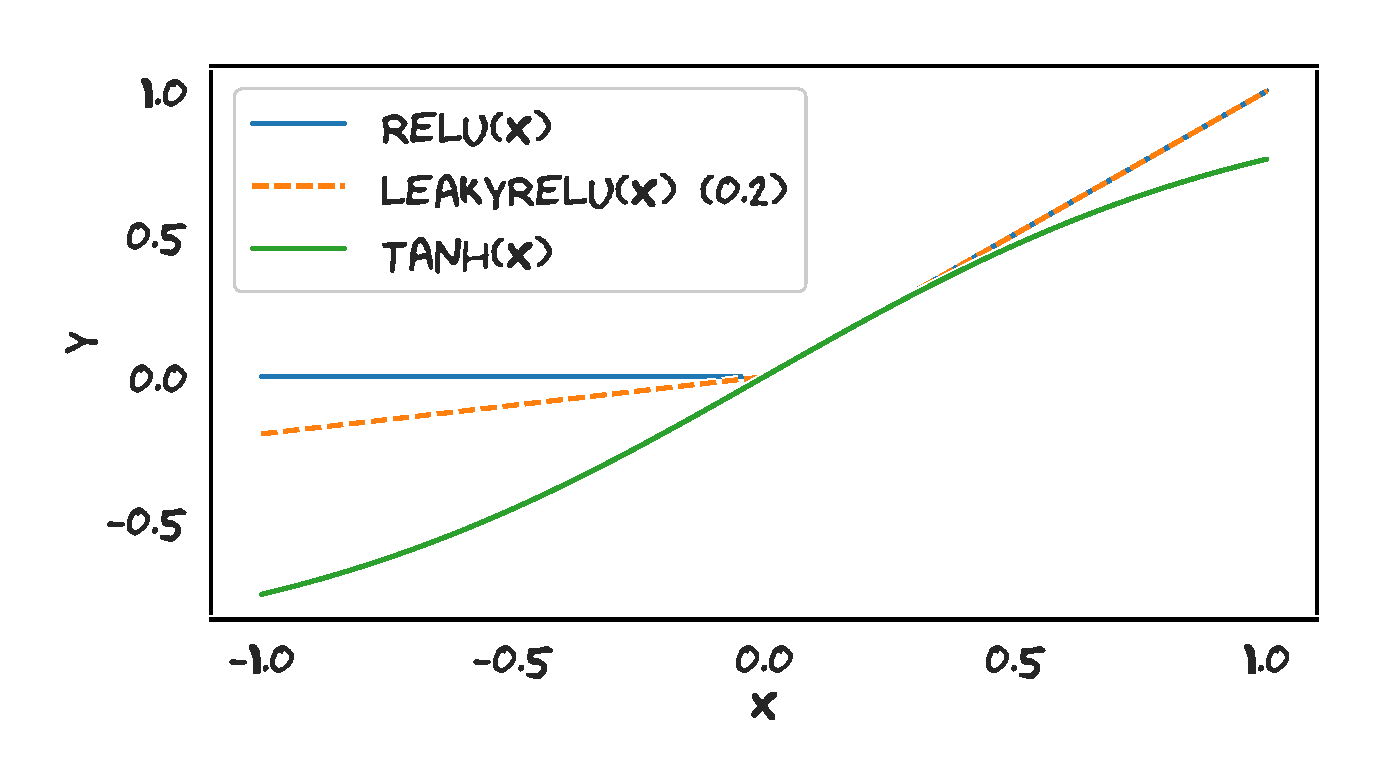
\includegraphics[width=\textwidth]{chapters/figures/relu_leakyrelu_example.eps}
    \caption{Activation output of \gls{relu}, leaky \gls{relu} and tanh.}
    \label{fig:leakyrelu}
\end{figure}


\subsection{Drop-out}\label{subsec:dropout}
Drop-out is a simple method for regularising \gls{dnn}. It is embedded into a layer and acts as a switch for turning off and on nodes. In other words, a probability (usually uniform) is added to all nodes in a layer where drop is wanted. When training, the probability is evaluated causing some nodes to \emph{turn off}. The intuition here is that by turning off some nodes (with some random probability), the combined model does not depend on a specific set of nodes to minimize the loss. This effectively reduces memorization and thus overfitting of the models \cite{Goodfellow-et-al-2016}. Drop-out is the core of the Bayesian approximation method proposed by \cite{Gal2015DropoutLearning}. Very briefly summarised it is utilizing the idea of keeping drop-out layers enabled during testing. By enabling drop-out during testing, an approximation of the posterior distribution can be sampled. The method proposes \gls{mc} sampling of the model, with drop-out enabled, to obtain an approximation of the posterior distribution. The method is based on the idea that overall variance of the underlying problem (given the model is well-tuned) is captured during learning, by the drop-out layers. Understanding the variation when predicting can offer metrics of uncertainty which is extremely useful when dealing with large \gls{dnn}.



\subsection{Batch Normalization}\label{subsec:batch_normalization}
Batch normalization is a key tool in the optimization of \gls{dnn}. The method is considered a so-called \emph{adaptive reparametrization} trick. It reduces the problem of only using the first-order gradient when updating multiple layers which would otherwise only converge using second-order statistics. In basic terms, batch normalization is a set of vectors containing the mean and the standard deviation of the activation output. These vectors are used for normalizing the activation output. Applying this to layers means that learning is stabilized around the distribution of the learning objective and not the expressiveness of the entire network. In other words, the information provided by the first-order gradient might be sufficient in many cases; however, when the \gls{dnn} increase in the number of the layers second-order statistics become non-negligible. Batch normalization improves the training of \gls{dnn} by accelerating it. It can mainly be seen as regularisation tool. It is commonly used instead of drop-out as it has been documented to improve performance in most \gls{dnn} \cite{Goodfellow-et-al-2016}.



\subsection{Upsample/Transposed Convolution}
The components of convolutional layers can effectively apply a set of dimensionality reduction techniques. In some modelling techniques, it is required to scale the resulting dimensionality back to the original input size. A component of building such models is by introducing so-called \emph{upsampling layers} or \emph{transposed convolutions} (also known as a deconvolution). Effectively the output of either method is the same but uses different modes of operation. 


\subsection{Learning Rate scheduler}\label{subsec:lr_scheduler}
The learning rate is a fundamental component of the weight update utilized in backpropagation. As seen from Eq. (\ref{eq:weight_update}) it defines the \emph{step size} of the gradient descent method. When utilizing \gls{dl} models, the weight space in which the gradient is computed tends to be complex. A key issue of training \gls{dl} models (or any \gls{ml} model for that matter) is the presence of local minima. As discussed in section \ref{subsec: optimizers}, the modern optimizers approach this by introducing terms when updating the weight. However, the learning rate is still considered an essential term for the overall weight update. Having too high learning rate effectively results in never reaching the global minima, while having a step size that is too low may result in no convergence within a feasible runtime. Thus, effectively controlling the parameter during training is the purpose of a so-called \emph{Learning Rate Scheduler}. By observing a metric of relevance, the properties of the learning rate can be evaluated while training. One approach is then to notice when no improvements take place during training and lower the learning rate as a result. This is also termed a \emph{Learning Rate Scheduler on Plateau}. An example can be seen in Fig. \ref{fig:learning_rate}, where learning has stagnated and is sequentially reduced.

\begin{figure}
    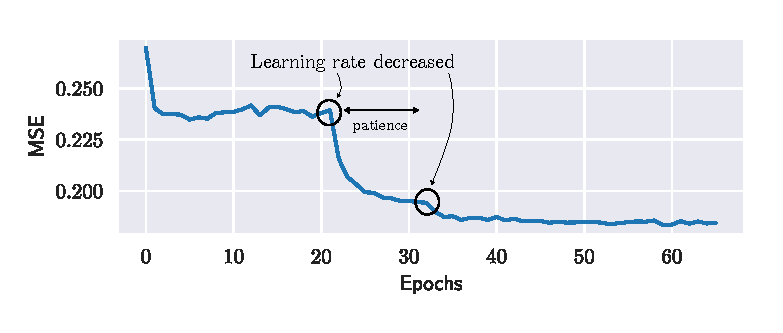
\includegraphics[]{chapters/figures/learningrate_scheduler_example.eps}
    \caption{Example of the training loss with a learning rate scheduler using a patience of 10 epochs before lowering the learning rate. }\label{fig:learning_rate}
\end{figure}

\subsection{Hyper-parameters}

The components of \gls{dnn} consists of many parameters. Such parameters are termed \emph{hyper-parameters} and effectively controls the complexity of the model. Hyper-parameters are fixed and not optimized during regular backpropagation optimization; thus, it is essential to evaluate how a given set of hyper-parameters perform. For the remainder of the dissertation, the notation for a \gls{nn} function $y(\cdot)$ with hyper-parameters is denoted as follows.

\begin{equation}
    t_n = y(x_n, \mathbf{w}, \theta) + \epsilon
\end{equation}

Where $t_n$ is the observation of the learning objective, $x_n$ are the input features, $\mathbf{w}$ are the adaptive weights updated during backpropagation, and $\theta$ denote the used hyper-parameters. An example of such hyper-parameter is the number of samples used in a pooling operation or the number of convolutions applied in the convolutional layer. Deep models are thus exposed to many tun-able parameters and require extensive experimentation to discover optimized hyper-parameters.

Fortunately, the world of computer science is exposed to a particular type of engineers that has the desire to automatize as many tasks as possible, which is also the case for discovering hyper-parameters. Principles of \gls{ml} and in general pattern recognition has successfully been applied to the discovery of the optimum hyper-parameters. Conventional methods include regular exhaustive grid search, random search and the more intelligent Bayesian Optimization which utilize Gaussian Process regression techniques \cite{YuHyper-ParameterApplications}. All of the said methods have been utilized throughout this dissertation.

Regardless of hyper-parameter optimization techniques, the training is still time-consuming. Thus it is necessary to consider relevant early-stopping criteria. Such approaches will be detailed later on for the specific applications.


\subsection{Implementation}
This section has contained some of the many components used in \gls{dnn}. The field is continuously evolving with new and improved methods for not only the processing of raw data like convolutional layers but also optimizers and methodologies for regularisation.  Implementing the state-of-the-art algorithms and structures is a time-consuming affair; however, several open-source libraries ensure that implementation is access-able to any enthusiast. In particular, a few libraries are considered the default selection, the most popular ones are 

\begin{itemize}
    \item TensorFlow \cite{tensorflow2015-whitepaper}
    \item PyTorch \cite{Paszke2017AutomaticPyTorch}
\end{itemize}

Both libraries are mostly a set of highly efficient low-level code written in the \texttt{C}- and \texttt{CUDA}-language. Ensuring ease of implementation is achieved by the abstraction of using the high-level language \texttt{python}. Both libraries enable standard components but also \gls{gpu} acceleration. TensorFlow is a long-standing library maintained by Google, but in recent years PyTorch (supported by subparts of Facebook) has seen an incredible rise in popularity due to the flat and transparent \gls{api} architecture. TensorFlow is not only a \gls{dl} library; it is an extensive collection of computational resources with deployment tools for production environments. The Pytorch library lacks most of these functionalities; however, the ease of implementation greatly out-weighs the benefits offered by TensorFlow. Both libraries have been utilized for the algorithm development in this dissertation. 

\section{Data needs}

Use of any learning algorithm requires data and observations. However, differences in the fundamental learning process (i.e. the family of the adaptive model) requires different kinds of data. For instance, supervised learning (as used predominantly throughout this dissertation) need large quantities of data when utilizing deeply nested models such as \gls{dnn}. Also, depending on the difficulties of the problem, the quantities of data may vary significantly. Obtaining such data is the first bottleneck to overcome. The fundamental properties of the chosen adaptive models put forward a different set of data requirements, and an overview of such requirements can be found in work such as \cite{RohAPerspective}. For example, acquiring necessary labels used for the classification of images is exhaustive and time-consuming, which has consequently lead to the rise of \emph{semi-supervised} approaches. Such methods use tricks and techniques to effectively improve the quantities of data without the need for obtaining additional. The authors show the pressing need for accurate and scalable data collection techniques, which is furthermore enabled by the promise of utilizing \gls{dl} for solving complex tasks. 

The expressiveness of the constructed models furthermore dictates the data requirements. In the case of complex models, the number of parameters and adaptive weights can easily surpass that of the available data points. The resulting models will fit to the observation noise, which is the definition of overfitting. If the data quantities are not constrained, proper regularisation is a necessity to find the optimal model complexity. 

Adaptive models associated with so-called \emph{Reinforcement learning} does not require massive data sets. It, however, requires integration with the actual system in which the problem or optimization task is present. Development of such a combination is time-consuming to engineer and must consider stringent requirements on not only latency but also processing power. Such requirements are usually a bottleneck for the integration of \emph{Reinforcement learning} solutions into real-world systems. For such reasons, simulation and emulation environments are essential for the future of \emph{reinforcement learning}. 

The methods and approaches used for obtaining the necessary data in order to apply the tools of \gls{dl} effectively are put forward in chapter \ref{ch:monster}. 

\section{Summary}
The world of \gls{ml} is massive. The toolbox is so deep and continually evolving that it is expected to get lost somewhere. However, a few terms and principles are expertly maintained and are regularly relevant for state-of-the-art algorithms. The content of this chapter is a brief introductory effort into the world of not only \gls{ml} but also \gls{dl}. To not further confuse the reader the content can be summarised to the following items

\begin{itemize}
    \item Adaptive models is a proven and necessary part of mobile communication systems. The basic principles of these models share the fundamental properties with Neural Networks. 
    \item Neural Networks is a powerful modelling technique that learns through cascaded structures of adaptive weights and non-linear transformations.
    \item \gls{dl} is a subfield of \gls{ml} that primarily utilize \gls{nn}-methodologies and definitions to process and learn from raw data.
    \item Open-source \emph{implementations} are paramount to the development of novel solutions.
    \item Data is the catalyst for novel \gls{dl}-based solutions.
\end{itemize}